As was noted in chapter~\ref{chp:introduction}, measurements of the \acs{rpnd}
been mostly limited to the afterglow plasma or time-integrated quantites.
Electric field measurements, either with capacitive probes or nonlinear
wave-mixing, thus far provide the only detail of the \acs{rpnd} during its
development. Though the electric field can be used to estimate electron
densities and reaction rates in the plasma, this requires a number of additional
assumptions.

As a result, there is a lack of reliable information on the particle properties
of the \acs{rpnd} during its development. That said, such information is
essential to confirming the present understanding of how these discharges
develop, optimizing them for specific applications, and providing important
benchmarks for numerical simulations. Therefore, a clear need exists for direct
measurements of the \acs{rpnd} particle properties.

Unfortunately, these measurements present a significant challenge for most
traditional plasma diagnostics. In most situations, the obvious choice would be
the Langmuir probe for its simplicity and ease of implementation. However, the
fast variations in the plasma potential, slow response of the ion, and high
collisionality all preclude this approach \cite{Lieberman2005}. Furthermore, any
physical probe would act as a significant perturbation in the system.

The logical alternative to physical probes is the use of optical diagnostics,
however these have their own associated difficulties. Electrons cannot be
studied by their emissions because, with the exception of bremsstrahlung, they
do not emit light. This leaves the light emitted from excited atoms. Atomic
emission spectroscopy can be used to measure many different plasma quantities,
from electron density, to local electric field strength. Unfortunately,
spontaneous emission can be a slow process compared to the development of the
\acs{rpnd}. For example, the fastest neutral helium transition in visible
wavelengths (3$^3$D$_3$-2$^3$P$_2^\cdot$) has a radiative life of 14 ns
\cite{Ralchenko2011}.

This suggests that instead of waiting for spontaneous emission to occur, it may
be better to use some form of active spectroscopy. Though the added complexity
of a well-characterized light source is undesirable, it adds several interesting
possibilities. For example, Thomson scattering provides a means for direct
interaction with electrons. In addition, it has a high spatial and temporal
resolution and is able to measure the electron density and temperature
simultaneously \cite{VanGessel2012}. However, the electron density limit of
$5\times10^{12}$ cm$^{-3}$ is too low for use with the \acs{rpnd} which may have
electron densities well below this \cite{Pai2009}.

With the ability to directly interact with electrons, the next alternative is to
target one of the excited states of helium. The lowest such state, the triplet
metastable (2$^3$S), resides at 19.82 eV. This is a relatively large energy gap
for an atom and indicates that virtually no such states should exist at room
temperature. The triplet metastable (and all higher-energy states in helium)
will be populated exclusively by energetic electrons. Therefore, a measurement
of the triplet metastable level is a useful indicator of the degree of helium
excitation as the \acs{rpnd} develops, and could potentially be used to infer
some properties of the electron population.

Perhaps the most straightforward approach to a measurement of the triplet
metastable density is with absorption spectroscopy. This approach has a long
history in the study of metastables in gas discharges, going back at least six
decades \cite{Phelps1953}. At its most basic, the technique involves
illuminating a plasma with light matching a transition between the metastable,
and some upper level and measuring the amount of light transmitted. The amount
of light transmitted is proportional to the metastable density integrated along
the path of the light traversing the plasma. The bandwidth of this measurement
is only limited by the time required for the light to pass through the plasma.

\section{Setup}

Traditionally, the light used in absorption spectroscopy has been supplied by
discharge tubes with the same gas as the system under study. Though
straightforward, this approach is limited by the luminosity of the discharge
tube, and the fact that the emitted radiation is isotropic. More recently,
Millard et al. noted that diode lasers provide a greatly improved light source
that provides simple spatial selectivity, at intensities which can easily exceed
the saturation limit \cite{Millard1998}.

As with the study by Millard et al., the decision was made to study the
transition from the triplet metastable to the 2$^3$P$^\mathrm{o}_{0,1,2}$ (at
approximately 1083 nm). This was done for several reasons. For one, the closest
helium transition is over 7 nm away, making it relatively isolated. In addition,
the different levels or values of $J$ are all within the tuning range of a
single diode. As each level has a different degeneracy, $g$, the strength of
absorption varies depending on the selected level. Thus, the absorption strength
can be increased for low densities, or decreased at high densities, improving
the dynamic range of the diagnostic.

The laser used was a distribute feedback laser diode, produced by Toptica, model
LD-1083-0070-DFB-1. The specified linewidth of the laser was 3 MHz, well below
the natural linewidth of the transition, 10.2 MHz. This situation can be
exploited to directly measure the gas temperature of the system, as will be seen
in the next section. The diode was rated for a total output power of 70 mW, with
a beam size of 1 mm by 3 mm and a vertical polarization. The diode was housed in
a Toptica DL DFB housing which incorporated the collimating optics. A Toptica
DCC 110 was used to provide current control for the diode laser, and a Toptica
DTC 110 was used to control the thermoelectric cooler for the diode.

The layout in figure~\ref{fig:laser}
\begin{figure}
  \centering
  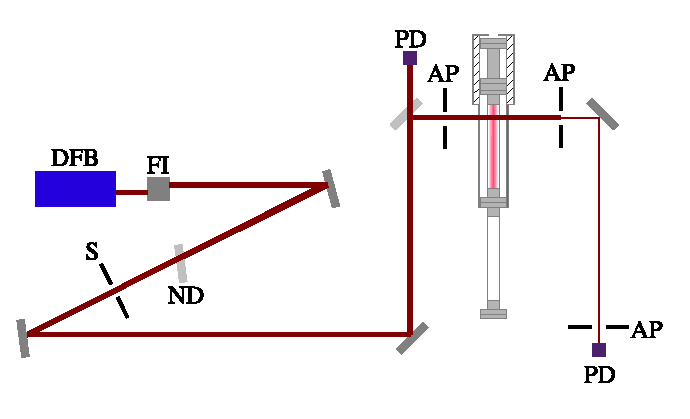
\includegraphics{./chapters/metastables/figures/laser.eps}
  \caption{Optical beam path of the laser in the absorption spectroscopy
  experiment. DFB - Distributed feedback laser diode; FI - Faraday isolator; ND -
  neutral density filter; S - shutter; PD - photodiode; AP - aperture.}
  \label{fig:laser}
\end{figure}
reflects the optical beam path used in the absorption experiment. The laser
light is produced by the distributed feedback laser diode (DFB). It then enters
a Electro-Optics Technology, Inc. Faraday isolator (FI) which prevents
back-reflections from entering the diode. Without the isolator in place, such
back-reflections can cause mode-hopping, resulting in unreliable tuning. The
laser intensity is then reduced by a neutral density filter (ND). Afterward, the
laser passes through a Vincent Associates electronic shutter (S). Then, the beam
is split by a Thorlabs BSF10-C beam sampler at a 45$^\circ$ angle. This reduced
the laser intensity below the saturation intensity (0.45 mW/cm$^2$) of the
transition. Collimation to a 1 mm circle, and alignment were provided by two
apertures (AP) on both sides of the discharge apparatus. The beam exiting the
apparatus was then sent through a final aperture to spatially filter plasma
emissions before being a Thorlabs F240SMA-780 collimation package was used to
couple the light into an optical fiber.

Behind the beam sampler was a Thorlabs DET300 germanium photodiode. The signal
from this photodiode was terminated at 1 M$\Omega$ and used to monitor the beam.
The opposite end of the optical fiber was affixed to a Thorlabs DET410 InGaAs
photodiode. The photodiode signal was amplified by a Femto HVA-200M-40-B voltage
amplifier before being sent to the oscilloscope. The time resolution of the
metastable measurements was determined by the InGaAs photodiode which had a
specified rise time of 5 ns.

In order to measure the absorption of the laser, it was first necessary to tune
the laser to the correct wavelength. This matter was complicated by the lack of
a wavemeter with sufficient precision and accuracy. As a result, a signal
generator was used to sweep the laser current so as to cover a frequency range
of 40 GHz. The temperature of the diode was then slowly adjusted until
absorption peaks corresponding to the 2$^3$S$_1$-2$^3$P$_{0,1,2}^\mathrm{o}$
transition were observed. The conversion between diode and wavelength was
measured with a CVI Melles Griot ET-25.4-10.00-30, solid dielectric etalon. It
was found that a temperature of 36$^\circ$ C and a current of 63 mA produced
resulted in an output wavelength of approximately 1082.9 nm.

As described in chapter~\ref{chp:experiment}, data acquisition was handled by a
LabView program, connected to the oscilloscope by GPIB\@. The auxiliary outputs of
the SRS SR850 lock-in amplifier were used to adjust the diode laser current (via
the DCC 110 module), and to trigger the electronic shutter. One of the auxiliary
inputs of the lock-in amplifier was used to read out the pressure from the
pressure controller.

Data were acquired for a range of pressure 0.3-16.0 Torr, and at three axial
locations: 5.08, 12.7, and 20.32 cm, relative to the glass-metal seal of the
anode. In reference to their location relative to the gas inlet these will be
referred to as the `upstream', `midstream', and `downstream' locations,
respectively. For each combination of location and pressure, absorption spectra
were measured over $\pm3.85$ GHz relative to the nominal transition frequency of
the 2$^3$S$_1$-2$^3$P$_0^\mathrm{o}$ transition at intervals of 154 MHz. The
absorption spectra were measured for time domains of $-300$-$1700$ ns relative
to the voltage pulse. Additional measurements were made at the midstream
position of the metastable densities from $-88$-$712$ $\mu$s in order to
investigate the loss mechanisms of the metastables.

The broadband electronic noise emitted by the fast pulses was a persistent issue
and presented one the greatest challenges to measurements during the \acs{rpnd}
development. As described above, the InGaAs photodiode was removed from the
immediate area surrounding the discharge by an optical fiber. The optical fiber
was routed through a small opening in a grounded metal box where both the
photodiode and the voltage amplifier resided. In addition, the DC power supply
of the voltage amplifier was connected to an outlet on a Tripp-lite Isobar
intended to provide additional isolation. The photodiode was connected directly
to the input terminal of the amplifier, while the amplifier was connected to a
BNC bulkhead adapter by a 10 cm length of RG 50/U. The final connection to the
oscilloscope was made by an additional 10 cm length of RG 50/U, running from the
BNC bulkhead connection.

Figure~\ref{fig:transmitted}
\begin{figure}
  \centering
  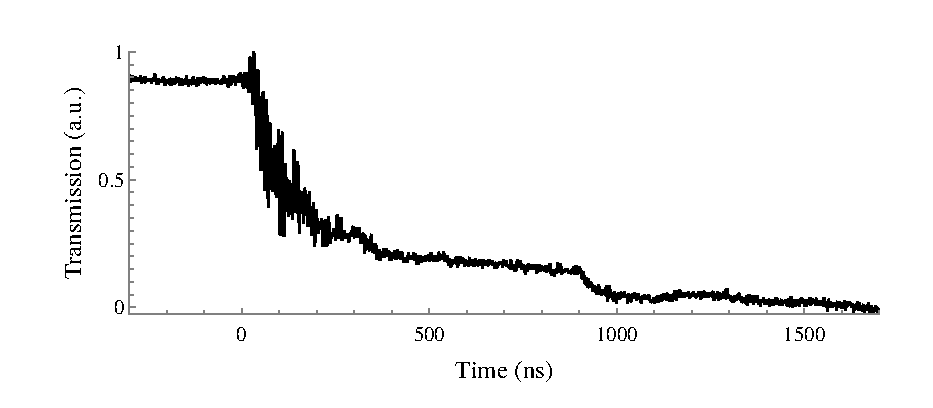
\includegraphics{./chapters/metastables/figures/transmitted.eps}
  \caption{Measurement of the transmitted laser light at the nominal transition
  wavelength at 4.0 Torr of helium.}
  \label{fig:transmitted}
\end{figure}
shows the transmission signal measured at the nominal transition wavelength for
a \acs{rpnd} in 4.0 Torr of helium. The signal is the average of 200 independent
pulses, further sampling had no appreciable effect on the waveform. As can be
seen, despite the efforts to limit the electrical interference, there is still a
substantial amount of noise present in the transmission signal. This is most
noticeable in the large ringing which occurs for the first 200 ns after the
voltage pulse. Without any kind of compensation, it would be impossible to
obtain reliable measurements of the transmission signal

\section{Absorption Analysis}

The noise produced by the \acs{rpnd} was relatively consistent between pulses
and over the duration of each experiment. As a result, it was possible to
correct for the electrical noise, as well as any spontaneous plasma emissions,
by measuring the signal from the photodiode in the absence of the laser. The
acquisition process proceeded as follows:
\begin{enumerate}
  \item Set desired laser wavelength.
  \item Wait 5 s for laser output to settle.
  \item Acquire 200 waveforms from photodiode.
  \item Close shutter.
  \item Acquire 200 waveforms from photodiode.
  \item Repeat
\end{enumerate}
The second set of waveforms was then subtracted from the first in the
post-processing stage. The effect of this subtraction can be seen in
figure~\ref{fig:contours}
\begin{figure}
  \centering
  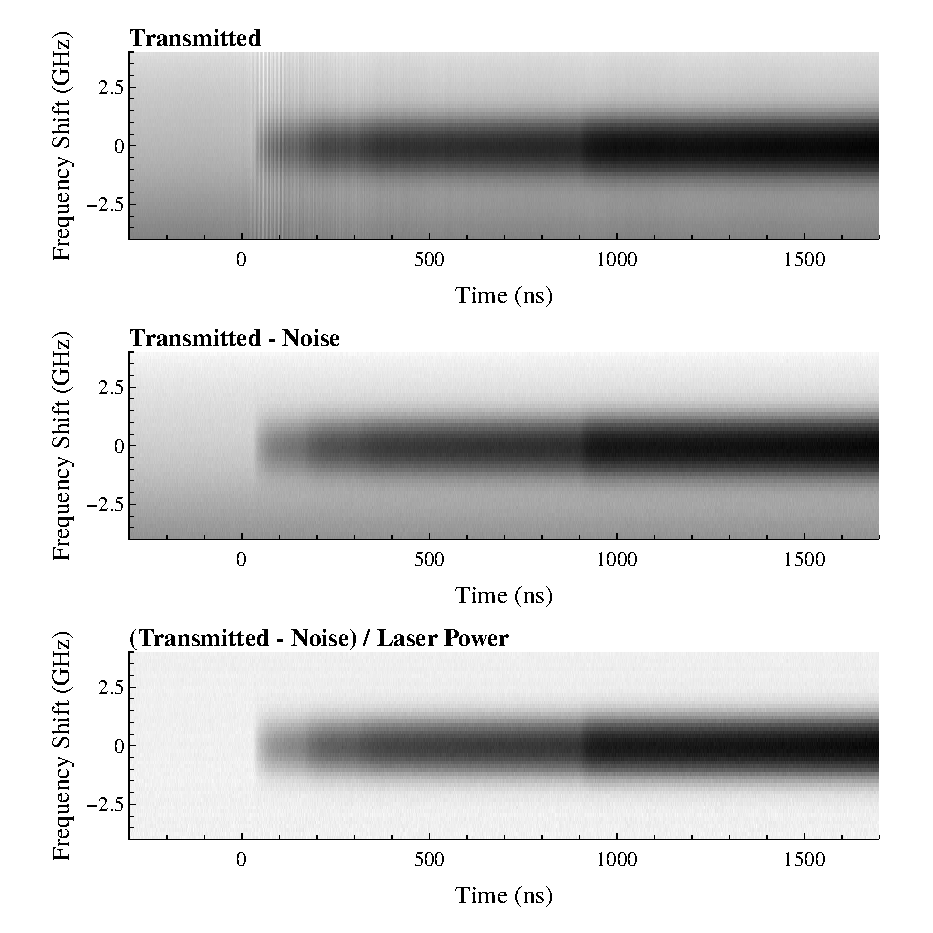
\includegraphics{./chapters/metastables/figures/contours.eps}
  \caption{Heatmaps of the transmitted laser signal for the 4.0 Torr condition at 
  various stages of post-processing.}
  \label{fig:contours}
\end{figure}
where the top heatmap shows the initial set of acquisitions with the laser on,
and the middle heatmap shows the transmitted signal with the noise subtracted.

As the laser diode current was changed in order to scan the wavelength across
the transition, the output power also changed by a small but significant amount.
The produces the gradient-like appearance of the top two plots in
figure~\ref{fig:contours}. In order to obtain a measurement of the unattenuated
laser power, the above acquisition procedure was repeated with the plasma off
for each operating condition. This made it possible to correct for the varying
laser power and to produce properly scaled transmission spectra.

These transmission spectra were then analyzed using a transmission model based
on the absorption cross sections described in chapter~\ref{chp:theory}. In a
one-dimensional system, the change in intensity of an incident photon field
(below the saturation limit), can be expressed as
\begin{equation}
  \frac{dI(x, \omega)}{dx} = -\sigma(\omega) N(x) I(x, \omega)
\end{equation}
where $I$ is the intensity of the photon field as a function of distance $x$,
$\omega$ is the frequency of the photons, $N$ is the density of the interacting
species, and $\sigma$ is the interaction cross section. This equation has the
simple solution,
\begin{equation}
  T(\omega) = \frac{I(x, \omega)}{I_0(\omega)}
            = \exp\left[-\sigma(\omega) \int_0^x N(x') dx'\right],
  \label{eq:transmitted}
\end{equation}
where $T$ is the transmitted intensity fraction, and $I_0$ is the initial
intensity of the photon field. The absorption can be trivially obtained from the
equation $A(\omega) = 1 - T(\omega)$.

For the purpose of analyzing the absorption, a quantity called the
line-integrated density will be defined. This is simply, $\nint = \int_0^x
N(x')dx'$. Equation~\ref{eq:absorb} can be used to determine the absorption
cross section. However, this requires that a lineshape be specified. If
possible, it is preferable to select either a purely Gaussian or purely
Lorentzian lineshape as the Voigt profile (equation~\ref{eq:voigt}) is
accompanied by a significantly larger computational cost. This can be determined
by a comparison of the relative widths of the different broadening mechanisms.
For a temperature of 300 K and a pressure of 8.0 Torr, it is found that $\dwd =
1.7$ GHz and $\dwa = 0.21$ GHz. Because neither broadening mechanism is
significantly dominant, the choice was made to analyze the data with a Voigt
profile, despite the added computational cost.

Equations~\ref{eq:transmitted},~\ref{eq:absorb}, and~\ref{eq:voigt} can be
combined to form a model equation for the transmitted spectrum. It can be seen
that only two unknowns exist: the gas temperature, $T_g$, and the
line-integrated density, $\nint$. For each time step, this model equation was
matched to the measured spectrum using the Levenburg-Marquardt algorithm
\cite{Marquardt1963} as implemented by the SciPy library \cite{Jones2001}.
During the matching process, it was observed that the diode current for which
absorption was optimized would shift over time. This was assumed to be the
result of small, long-term variations in the diode temperature that were not
adequately compensated for by the temperature control system. This corresponded
to a frequency drift of $\pm60$ MHz between experiments. For each experiment,
this frequency offset was measured for the spectrum with the largest absorption
signal and was then used to correct the analysis of all other spectra.

\section{Results}

The matching algorithm proved robust enough to automatically match the
transmission spectrum at each time step with no user intervention.
Figure~\ref{fig:matching}
\begin{figure}
  \centering
  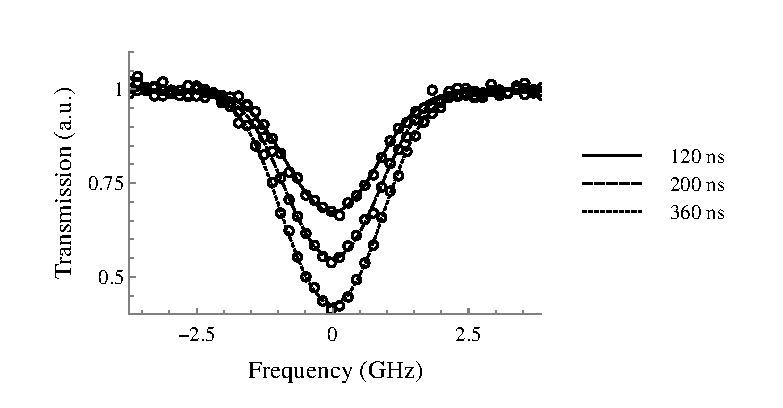
\includegraphics{./chapters/metastables/figures/matching.eps}
  \caption{Comparison of the measured transmission profile (open symbols) and
  the computer-generated matches for at several different times for the 4.0 Torr
  operating condition.}
  \label{fig:matching}
\end{figure}
shows three examples of the measured transmission spectra along with the
computer-generated matches. The measure data far from the peak coincide almost
perfectly with an unabsorbed signal. In addition, the spectrum at 120 ns shows
no evidence of the noise caused by the discharge. The variation in the baseline
transmission signal is approximately 0.02. This sets a minimum line-integrated
detection limit of approximately $3.0 \times 10^{14}$ m$^{-2}$, though the
actual value will depend to some extent on the pressure and temperature.

\subsection{Temperatures}

The temperatures calculated for the metastables from the laser-absorption
spectroscopy are shown in figure~\ref{fig:temperatures}.
\begin{figure}
  \centering
  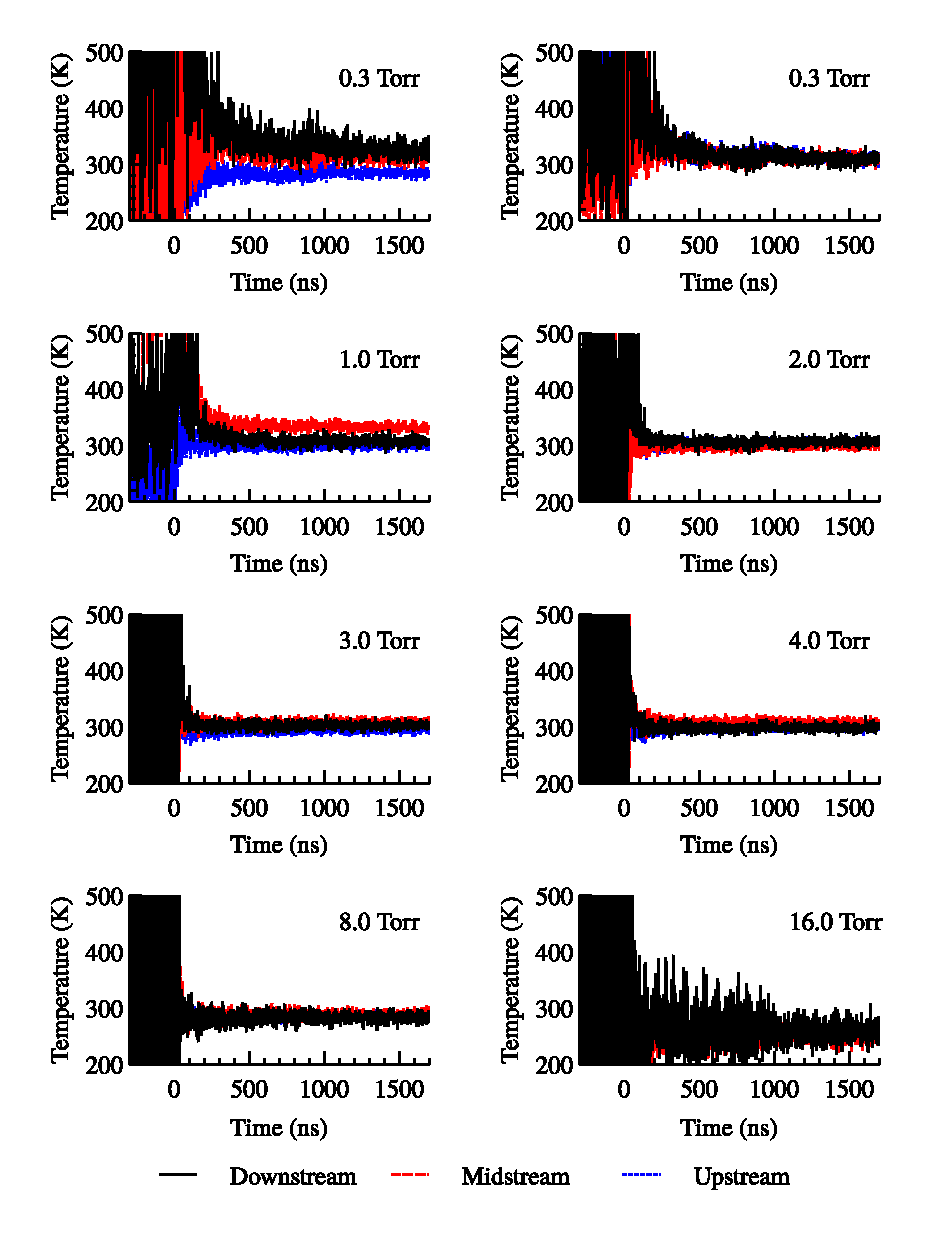
\includegraphics{./chapters/metastables/figures/temperatures.eps}
  \caption{Plot of the gas temperatures at each of the operating
  pressures and each axial location as a function of time.}
  \label{fig:temperatures}
\end{figure}
Prior to the pulse, the temperature estimates are subject to large variations.
This is a result of the low metastable densities which precede the pulse.
Without a substantial metastable population to work with the matching algorithm
has difficult discriminating between a combination of low temperatures and low
densities (a small narrow absorption spectrum) versus high temperatures and high
densities (a very broad absorption spectrum).

It is not possible to precisely calculate the error for the matching process at
each time step, however it is possible to estimate the standard deviation. In
all cases, the estimated standard deviation is less than 10 K by the end of the
measurement period. Overall, no significant temperature trends appear with
regard to time, axial location or pressure. Furthermore, the temperature of the
gas in the \acs{rpnd} appears to remain at room temperature, approximately 300
K, for all conditions.

This lack of change contrasts with previous studies of gas heating in
\acs{rpnd}s and \acs{fiws} \cite{Popov2011, Zuzeek2011, Pai2009}. Likewise,
recent measurements of the optical emissions from a \acs{rpnd} in air showed
significant heating, see appendix~\ref{chp:oes}. 

with \acs{rpnd}s and \acs{fiw}s in molecular
gases

\subsection{Line-integrated Densities}

\begin{figure}
  \centering
  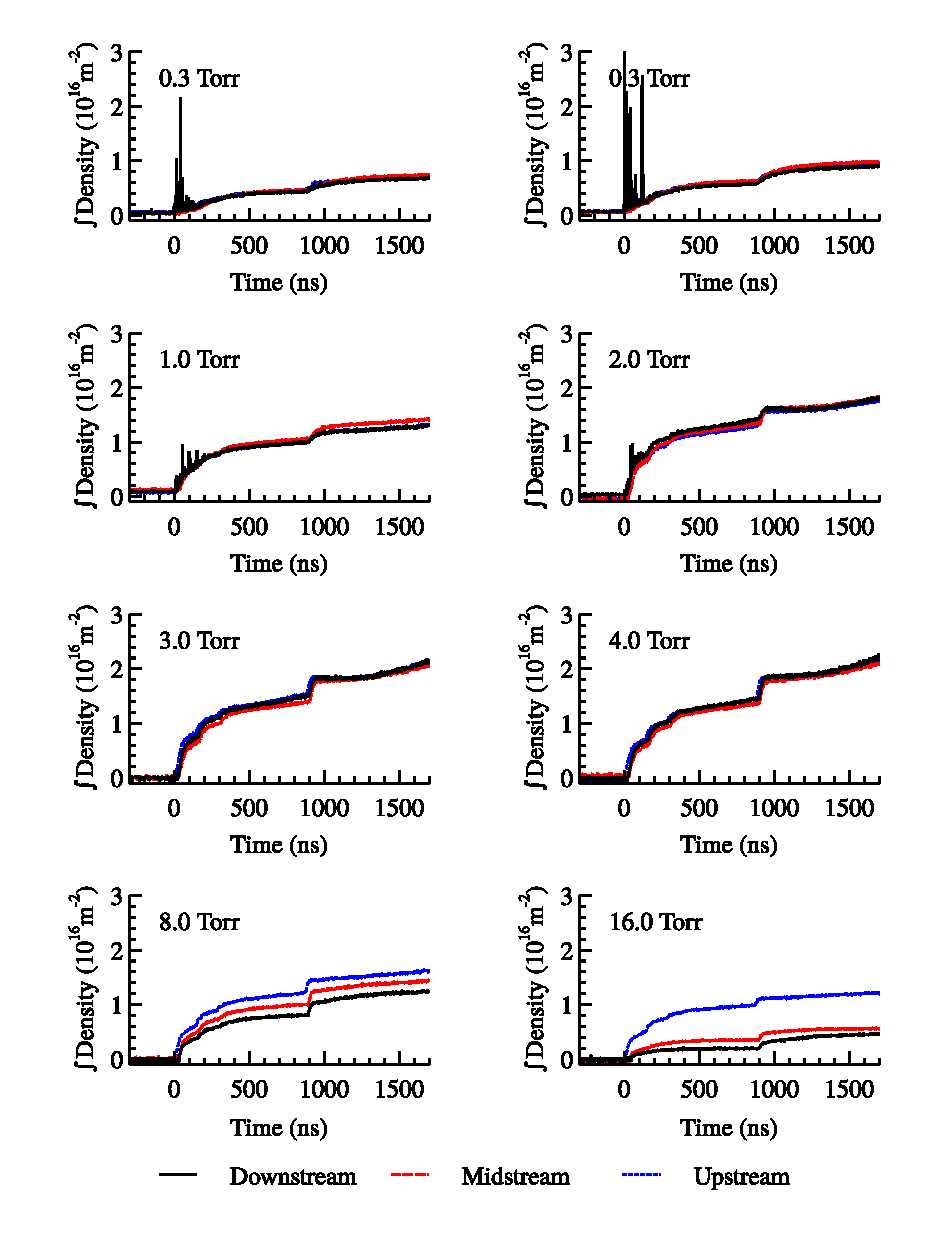
\includegraphics{./chapters/metastables/figures/metastables.eps}
  \caption{Plots of the line-integrated metastable densities at each of
  the operating pressures and each axial location as a function of
  time.}
  \label{fig:metastables}
\end{figure}
